% THIS IS SIGPROC-SP.TEX - VERSION 3.1
% WORKS WITH V3.2SP OF ACM_PROC_ARTICLE-SP.CLS
% APRIL 2009
%
% It is an example file showing how to use the 'acm_proc_article-sp.cls' V3.2SP
% LaTeX2e document class file for Conference Proceedings submissions.
% ----------------------------------------------------------------------------------------------------------------
% This .tex file (and associated .cls V3.2SP) *DOES NOT* produce:
%       1) The Permission Statement
%       2) The Conference (location) Info information
%       3) The Copyright Line with ACM data
%       4) Page numbering
% ---------------------------------------------------------------------------------------------------------------
% It is an example which *does* use the .bib file (from which the .bbl file
% is produced).
% REMEMBER HOWEVER: After having produced the .bbl file,
% and prior to final submission,
% you need to 'insert'  your .bbl file into your source .tex file so as to provide
% ONE 'self-contained' source file.
%
% Questions regarding SIGS should be sent to
% Adrienne Griscti ---> griscti@acm.org
%
% Questions/suggestions regarding the guidelines, .tex and .cls files, etc. to
% Gerald Murray ---> murray@hq.acm.org
%
% For tracking purposes - this is V3.1SP - APRIL 2009

\documentclass{acm_proc_article-sp}

\usepackage[breaklinks,colorlinks=true,linkcolor=black,urlcolor=black,citecolor=black]{hyperref}
%\usepackage{url}

\begin{document}

\title{Computer Secondary Storage}
\subtitle{Seminar: Use of Modern Hardware in Big Data Processing}
%
% You need the command \numberofauthors to handle the 'placement
% and alignment' of the authors beneath the title.
%
% For aesthetic reasons, we recommend 'three authors at a time'
% i.e. three 'name/affiliation blocks' be placed beneath the title.
%
% NOTE: You are NOT restricted in how many 'rows' of
% "name/affiliations" may appear. We just ask that you restrict
% the number of 'columns' to three.
%
% Because of the available 'opening page real-estate'
% we ask you to refrain from putting more than six authors
% (two rows with three columns) beneath the article title.
% More than six makes the first-page appear very cluttered indeed.
%
% Use the \alignauthor commands to handle the names
% and affiliations for an 'aesthetic maximum' of six authors.
% Add names, affiliations, addresses for
% the seventh etc. author(s) as the argument for the
% \additionalauthors command.
% These 'additional authors' will be output/set for you
% without further effort on your part as the last section in
% the body of your article BEFORE References or any Appendices.

\numberofauthors{2} %  in this sample file, there are a *total*
% of EIGHT authors. SIX appear on the 'first-page' (for formatting
% reasons) and the remaining two appear in the \additionalauthors section.
%
\author{
% You can go ahead and credit any number of authors here,
% e.g. one 'row of three' or two rows (consisting of one row of three
% and a second row of one, two or three).
%
% The command \alignauthor (no curly braces needed) should
% precede each author name, affiliation/snail-mail address and
% e-mail address. Additionally, tag each line of
% affiliation/address with \affaddr, and tag the
% e-mail address with \email.
%
% 1st. author
\alignauthor
Sascha K{\"o}nigsberg\\
       \affaddr{Technische Universit{\"a}t M{\"u}nchen}\\
       \email{sascha.koenigsberg@tum.de}
% 2nd. author
\alignauthor
Claus Strasburger\\
       \affaddr{Technische Universit{\"a}t M{\"u}nchen}\\
       \email{claus@strasburger.de}
}

\date{20 May 2014}

\maketitle
\begin{abstract}
This report contains a summary of developments in computer secondary storage, particularly in big data server environments. We describe the history of \emph{Hard Drives} and \emph{Solid State Disks} and list tradeoffs and considerations of the currently available options. We present \emph{Phase Change Memory}, a possible alternative for the future of secondary storage, its history and current state of research. We provide a summary of the presented techniques and trends.%% fazit?
\end{abstract}


%%TODO categories!!
% A category with the (minimum) three required fields
\category{H.4}{Information Systems Applications}{Miscellaneous}
%A category including the fourth, optional field follows...
\category{D.2.8}{Software Engineering}{Metrics}[complexity measures, performance measures]

\section{Introduction}

\section{History of storage drives}

\subsection{Hard Disk Drives}

\subsection{Solid State Disks}

\section{Advantages and disadvantages of SSDs compared to HDDs}

\section{SSD challenges}

Solid State Drives pose many difficult challenges to both their manufacturers and users. Despite the superior theoretical access time and read/write bandwidth of NAND flash, the inherent limitations of NAND flash memory make development and use of SSD much more difficult and completely different to regular hard disk drives.

\subsection{Hardware Limits}
NAND flash has two major limits: Block erasure and write cycles (\emph{Memory wear}). Other limitations include Bit Corruption and Read Disturb

\subsubsection*{Block Erasure}
Because of the higher current which is necessary to release the trapped charge in a flash memory cell compared to charging a cell, this process is done in blocks of cells, called \emph{Erase Blocks}. Most current Solid State Disks use blocks of 256 pages or more \cite{codecapsule2014coding}.
This means that to write to a page which was previously written and subsequently marked as unused, either all pages on the same erase block have to be marked unused too, or currently in use pages have to be copied to another block. It is not until this has been done that the block can be erased. This process is called \emph{Garbage Collection}.

\subsubsection*{Limited Write Cycles}
When writing to a flash cell, charge is captured in it, similiar to a capacitor. %TODO similiar? the same? hmm.
However, when erasing it, not all charge is released. Some electrons get trapped in the gate, which leads to a point where the potential of an uncharged cell is nondistinguishable from that of a charged cell. This phenomenon, known as \emph{Memory wear}, occurs earlier in multi level cells, since the cell is unusable as soon as the zeroth level is indistinguishable from the first level.
Current SLC NAND flash cells have lifetimes from 100 thousand program/erase (\emph{P/E}) cycles to one million before becoming useless, while multi level or triple level cells have 3 thousand to ten thousand cycles.

\subsubsection*{Bit Corruption}
Raw flash memory is prone to random bit errors, because of charge leaking in and out of storage cells. Error correcting codes (\emph{ECC}), as well as error detecting codes (such as Cyclic Redundancy Check, \emph{CRC}) are used to find and possibly correct errors without silently corrupting data.

\subsubsection*{Read Disturb}
Another phenomenon in NAND flash is called \emph{Read Disturb}. When a cell is accessed many times without being erased, trapped charge can build up in nearby cells, causing them to flip their status if they were uncharged before. %TODO sicher, dass sich etwas aufbaut und nichts abbaut?
This happens after about one million reads without erase in single level cells and after 100 thousand reads for multi level cells.
\\
To prevent read disturb from corrupting data, SSD controllers keep count of how many times a page was read since the last erase cycle. When a predefined critical read limit is approached, the data is moved or re-programmed.

\subsection{Controller Firmware Challenges}
SSD controllers have to do a lot of bookkeeping to prevent the underlying flash memory from corrupting data or deteriorating. Errors or oversights in controller firmware programming can lead to drastically reduced performance, data loss or silent data corruption.

\subsubsection*{Garbage Collection}
In order to write data to flash memory, free pages have to be available. SSD controllers use Over-Provisioning (\emph{OP}) to keep the number of unwritten pages high during burst writes, but if more data is to be written than free pages are available, or when invalidated pages need to be reclaimed, garbage collection is necessary. In this process, the controller copies still-valid pages out of blocks containing many invalid pages, only then the whole block can be erased. As the number of invalid or free pages --- to the operating system these are known as \emph{free} space --- decrease, more garbage collection and copying of pages in use has to be done in order to ensure available pages on write requests.

\subsubsection*{Wear Leveling}


\subsubsection*{Write Amplification}
Summing up these techniques used by the controller, write accesses to the device --- or in the case of Read Disturb mitigation read accesses, too --- lead to more data being written than requested by the operating system. % small writes

\subsection{Software Challenges}
Even though SSD manufacturers go to great lengths to ensure optimal performance and data integrity, there are still considerations necessary for system architects and developers when building software or systems using SSDs. Blindly following current usage patterns established for rotating media will lead to bad performance, possibly worse than with hard drives, sudden performance drop or high device failure rate.

\subsubsection*{Random Writes}
Even though SSDs have no mechanical parts, sequential writes will still be faster than small writes. Applications have to be careful to try and write in as big blocks as possible, since the smallest written unit will always be the page size (currently 8 to 16 KiB). Small, random writes, such as those produced by a conventional Relational Database Management System (\emph{RDBMS}) like PostgreSQL or MySQL, will cause rapid allocation of many pages, which then need to be garbage collected. As soon as the SSD controller runs out of overprovisioned pages, garbage collection will be necessary and drastically slow down the device. The effective Write Amplification will be very high (depending on the write sizes and their ratio to the page and block sizes), also leading to faster memory degradation and therefore a high disk failure rate.

\subsubsection*{TRIM}
\emph{TRIM} is an ATA command used to mark unused pages. Conventional spinning hard drives have and need no concept of used or unused storage, since all they do is write and read. With SSDs, the controller needs to know what data is actually valid, otherwise it will do bookkeeping for data no longer referenced by the file system. Also, this storage space cannot be used by the controller to perform garbage collection, wear leveling or other optimization techniques and consequently slows down operation.
\\
To resolve this, the TRIM command has been introduced to the ATA specification to allow the operating system or file system to inform the drive when files are being unlinked. The SSD controller can then reclaim the now free space and use it at will.
\\
The lack of TRIM support was an issue when first introducing SSDs, it has however been implemented in all major operating systems since 2011. Still, some combinations of operating and file systems (for example NTFS-3g on Linux or Android before 4.3) might lack TRIM support and therefore cannot take full advantage of SSD speeds.

\section{Parallel access mechanisms}

\subsection{B-Tree Layer for Flash Memory Storage Systems}

\cite{wu2007efficient}

\subsection{Fractal Prefetching B$^{+}$-Trees}

\cite{chen2002fractal}

\subsection{?} % microsoft case study?

\subsection{Flash as Cache Extension (\subsecit{FaCE})}

\cite{kang2012flash}

\section{Current Research}

\subsection{Phase Change Memory (\secit{PRAM})}

\subsection{Self-healing NAND Flash Memory}
\cite{wu2011exploiting}
\cite{chen2013dheating}

\section{Future Trends}
% also note: PCIe SSDs have no hotswap mechanism! terrible for servers!


\balancecolumns
%% examples begin

\begin{table*}
\centering
\caption{Some Typical Commands}
\begin{tabular}{|c|c|l|} \hline
Command&A Number&Comments\\ \hline
\texttt{{\char'134}alignauthor} & 100& Author alignment\\ \hline
\texttt{{\char'134}numberofauthors}& 200& Author enumeration\\ \hline
\texttt{{\char'134}table}& 300 & For tables\\ \hline
\texttt{{\char'134}table*}& 400& For wider tables\\ \hline\end{tabular}
\end{table*}
% end the environment with {table*}, NOTE not {table}!

\begin{figure}
\centering
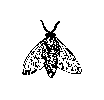
\epsfig{file=fly.eps}
\caption{A sample black and white graphic (.eps format).}
\end{figure}

\begin{figure}
\centering
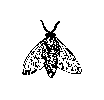
\epsfig{file=fly.eps, height=1in, width=1in}
\caption{A sample black and white graphic (.eps format)
that has been resized with the \texttt{epsfig} command.}
\end{figure}
%examples end

%
% The following two commands are all you need in the
% initial runs of your .tex file to
% produce the bibliography for the citations in your paper.
\bibliographystyle{abbrv}
\bibliography{secondary-storage}  % sigproc.bib is the name of the Bibliography in this case
% You must have a proper ".bib" file
%  and remember to run:
% latex bibtex latex latex
% to resolve all references
%
% ACM needs 'a single self-contained file'!
%

\balancecolumns
\end{document}
